\documentclass[12pt,reqno]{article}
\usepackage[dutch]{babel}
\usepackage[margin=1.3in]{geometry}
\usepackage{amsmath}
\usepackage{amssymb}
\usepackage{amsthm}
\usepackage{color}
\usepackage{tikz}
\usepackage{url}

\title{\textbf{Congruente getallen}\\
		\small{eerste versie begeleider}}
\author{
	\begin{tabular}{ l l }
		Lotte Bruijnen, & 4297652 \\
		Daan van Laar, & 5518741 \\
		Suzanne Vincken, & 4273338
	\end{tabular}\\\\
	Onder begeleiding van: Carel Faber, UU
}
\date{04-01-2016}

\newcommand*{\NN}{\ensuremath{\mathbb{N}}}
\newcommand*{\ZZ}{\ensuremath{\mathbb{Z}}}
\newcommand*{\QQ}{\ensuremath{\mathbb{Q}}}
\newcommand*{\RR}{\ensuremath{\mathbb{R}}}
\newcommand*{\CC}{\ensuremath{\mathbb{C}}}

\renewcommand{\qedsymbol}{$\blacksquare$}

\theoremstyle{theorem}
\newtheorem{theorem}{Stelling}
\newtheorem{lemma}[theorem]{Lemma}
\newtheorem{proposition}[theorem]{Propositie}
\newtheorem{corollary}[theorem]{Gevolg}

\theoremstyle{definition}
\newtheorem{example}[theorem]{Voorbeeld}
\newtheorem{definition}[theorem]{Definitie}
\newtheorem{remark}[theorem]{Opmerking}


\begin{document}	
	\begin{titlepage}
		\maketitle
		\thispagestyle{empty}
		\begin{figure*}[h!]
			\centering
			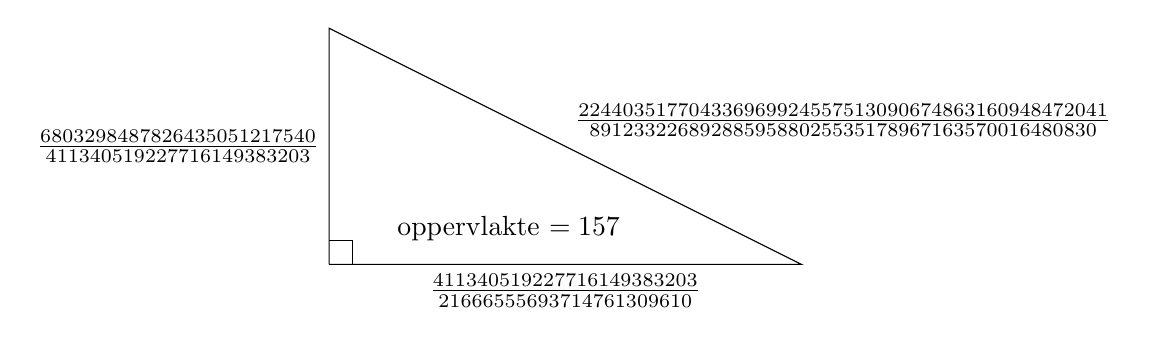
\begin{tikzpicture}[xscale=6, yscale=3]
			\coordinate (O) at (0,0);
			\coordinate (A) at (1,0);
			\coordinate (B) at (0,1);
			\coordinate (M) at (0.38, 0.15);
			\draw (O) -- node[auto,swap]{$\frac{411340519227716149383203}{21666555693714761309610}$} 
			(A) -- node[auto,swap]{$\frac{224403517704336969924557513090674863160948472041}{8912332268928859588025535178967163570016480830}$}
			(B) -- node[auto,swap]{$\frac{6803298487826435051217540}{411340519227716149383203}$} (O);
			\draw (M) node[auto]{oppervlakte $=157$};
			\coordinate (X1) at (0,0.1);
			\coordinate (X2) at (0.05,0.1);
			\coordinate (X3) at (0.05,0);
			\draw (X1) -- (X2) -- (X3);
			\end{tikzpicture}
		\end{figure*}
	\end{titlepage}

	\allowdisplaybreaks
	
	\section{Inleiding}
	We hebben onderzoek gedaan naar congruente getallen om onze kennis te verbreden. Het is een onderwerp uit de getaltheorie. In dit werkstuk zullen we vertellen wat we hebben gevonden.
	
	In hoofdstuk 2 zullen we Pythagore\"ische drietallen en congruente getallen behandelen. We zullen definities geven en we leggen uit wat deze twee onderwerpen met elkaar te maken hebben. Daarna, in hoofdstuk 3, zullen we een aantal voorbeelden geven van congruente getallen. Hoofdstuk 4 zal gaan over het vinden van congruente getallen. Hoe vinden we alle getallen die congruent zijn? In het laatste hoofdstuk, hoofdstuk 5, zullen we kijken naar presentaties van congruente getallen. Dit heeft te maken met Pythagore\"ische drietallen. Als afsluiting zullen we een samenvatting geven van alles wat we hebben behandeld.
	
	
	%\beginsection{Daan}
	\section{Pythagore\"ische drietallen en Congruente getallen}
	%Wat is een Pythagoreisch drietal?
	%Wat is een congruent getal?
	%  - algebraische definitie + bewijs
	%  - meetkundige definitie
	%  - definitie primitieve congruente getallen: Een kwadraatvrij congruent getal
	%Er schijnt een stelling te zijn die alle Pythagoreïsche drietallen classificeert. Als je die kan vinden, kan je het die even noemen.
	Eerst zullen we kijken naar de definitie van congruente getallen. Er bestaan echter meerdere definities. We zullen er hier twee behandelen.\\
	
	Ten eerste kijken we naar de meetkundige definitie uit \cite{Oort}[p.3]:	
	
	\begin{definition}\label{def:meetkunde}
		Een positief geheel getal $n$ heet een congruent getal als er een rechthoekige driehoek bestaat met lengtes van zijden in $\QQ_{>0}$ en met oppervlak gelijk aan $n\in\ZZ$. Noem de lengtes van de zijden $x,y,z\in\QQ$; met behulp van de stelling van Pythagoras zien we:
		\begin{figure*}[h!]
			\centering
			\begin{tikzpicture}[xscale=6, yscale=3]
			\coordinate (O) at (0,0);
			\coordinate (A) at (1,0);
			\coordinate (B) at (0,1);
			\draw (O) -- node[auto,swap]{$x$} 
			(A) -- node[auto,swap]{$z$}
			(B) -- node[auto,swap]{$y$} (O);
			\coordinate (M) at (1.5, 0.5);
			\draw (M) node[auto]{$x\cdot \dfrac{y}{2} = n$};
			\coordinate (N) at (1.5, 0.25);
			\draw (N) node[auto]{$x^2 + y^2 = z^2$};
			\coordinate (X1) at (0,0.1);
			\coordinate (X2) at (0.05,0.1);
			\coordinate (X3) at (0.05,0);
			\draw (X1) -- (X2) -- (X3);
			\end{tikzpicture}
		\end{figure*}
	\end{definition}
	We zien dat hier een congruent getal $n$ wordt gegeven als de oppervlakte van een rechthoekige driehoek met zijn zijden in $\QQ$. We kunnen conguente getallen ook bekijken via een algebra\"{i}sche benadering. De volgende definitie komt van \cite{Oort}[p.3].

	\begin{definition}\label{def:algebra}
		Een positief geheel getal $n$ heet een congruent getal als er bestaat een $\delta\in\QQ$ zodanig dat
		\begin{align*}
		\delta^2 - n,\quad \delta^2,\quad \delta^2 + n
		\end{align*}
		kwadraten zijn in $\QQ$.
	\end{definition}	
	Een getal dat aan deze definitie voldoet is het getal 5. We nemen $\delta = \frac{41}{12}$. Dan geldt:
	\begin{align*}
	\delta^2 &= \left( \frac{41}{12} \right)^2 \in\QQ\\
	\delta^2 - n &= \frac{1681}{144} - 5 = \frac{961}{144} = \left( \frac{31}{12}\right)^2 \in\QQ\\
	\delta^2 + n &= \frac{1681}{144} + 5 = \frac{2401}{144} = \left( \frac{48}{12}\right)^2 \in\QQ
	\end{align*}
	Hieruit volgt dus dat $5$ een conguent getal is. \\
	
	%Een andere manier om congruente getallen te defini\"{e}ren is door er op een meetkundige manier naar te kijken. Echter, voor die definitie is het handig om eerst te kijken naar Pythagore\"ische drietallen. \\
	
	%Dit straks verwijderen en de definities weer omdraaien.
	Bij de eerste definitie maken we gebruik van Pythagore\"ische drietallen. Daar zullen we nu wat meer over uitleggen.\\
	
	De geschiedenis van Pythagore\"ische drietallen begint bij het vermoeden van Fermat. Dit vermoeden ziet er als volgt uit:
	\begin{align}
	x^n + y^n = z^n \qquad \text{met} \qquad n \in \NN.
	\end{align}
	Fermat vermoedde dat voor $n \geq 3$ er alleen triviale oplossingen bestaan voor (1). Dat wil zeggen, $\forall (x,y,z) \in \ZZ^3$ en $x^n + y^n = z^n$ met $n \geq 3$, geldt $x \cdot y \cdot z = 0$. \\
	Wij zijn echter vooral ge\"interesseerd in het geval waarbij $n=2$ en alle niet triviale oplossingen van de vergelijking $x^2 + y^2 = z^2$. Deze oplossingen noteren we als $(x,y,z)$ en we noemen deze oplossingen Pythagore\"ische drietallen. Dit komt omdat het vermoeden van Fermat met $n=2$ de stelling van Pythagoras is. De niet-triviale oplossingen $(x,y,z)$ van $x^2 + y^2 = z^2$ vormen dan ook een rechthoekige driehoek waarbij $z$ de schuine zijde is. Een simpel voorbeeld van een Pythagore\"isch drietal is $(3,4,5)$, want $3^2 + 4^2 = 9 + 16 = 25 = 5^2$. \\
	Een speciaal soort Pythagore\"isch drietal is het zogenaamde primitieve Pythagore\"ische drietal. Dit is een Pythagore\"isch drietal $(x,y,z)$ waarvoor ook geldt dat $ggd(x,y)=1$.
	{\color{red}Bewijs dat ggd(x,z) en ggd(y,z) ook 1 zijn. Nog veel meer bewijzen over ppd's.}
	%Tweede definitie congruente getallen
	
	%Dat ding uit het boek, zie whatsapp
	\begin{proposition}
		\cite{Koblitz}[p.4, vertaald] Laat $n$ een vast kwaadraatvrij positief getal zijn. Laat $x,y,z,\delta \in\QQ$ met $x<y<z$. Er is een \'e\'en op \'e\'en relatie tussen rechthoekige driehoeken met zijden $x$ en $y$, schuine zijde $z$ en oppervlakte $n$, en getallen $\delta$ waarvoor geldt dat $\delta$, $\delta +n$ en $\delta -n$ de kwadraten zijn van een rationeel nummer. De correspondentie is:
		\begin{align}
		x,y,z &\rightarrow \delta = \left( \frac{z}{2} \right)^2 \\
		\delta &\rightarrow x=\sqrt{\delta+n} - \sqrt{\delta-n},\quad y = \sqrt{\delta+n}+\sqrt{\delta-n},\quad z = 2\sqrt{\delta}.
		\end{align}
		In het bijzonder, $n$ is een congruent getal dan en slechts dan als er bestaat een $\delta$ zodat $\delta$, $\delta+n$ en $\delta-n$ kwadraten van rationele nummers zijn.
	\end{proposition}
	
	
	%\endsection{Daan}


	\section{Voorbeelden}
	De eerste negentien congruente zijn: $5$, $6$, $7$, $13$, $14$, $15$, $21$, $22$, $23$, $29$, $30$, $31$, $34$, $37$, $38$, $39$, $41$, $46$, $47$. \cite{Coates}[p.19] We zullen hieronder drie voorbeelden geven.\\
	\\
	Het kleinste congruente getal is $5$. Dat is de driehoek met de volgende zijden:
	\begin{figure*}[h!]
		\centering
		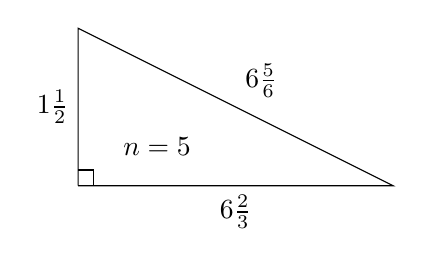
\begin{tikzpicture}[xscale=4, yscale=2]
		\coordinate (O) at (0,0);
		\coordinate (A) at (1,0);
		\coordinate (B) at (0,1);
		\coordinate (M) at (0.25, 0.25);
		\draw (O) -- node[auto,swap]{$6\frac{2}{3}$} 
		(A) -- node[auto,swap]{$6\frac{5}{6}$}
		(B) -- node[auto,swap]{$1\frac{1}{2}$} (O);
		\draw (M) node[auto]{$n=5$};
		\coordinate (X1) at (0,0.1);
		\coordinate (X2) at (0.05,0.1);
		\coordinate (X3) at (0.05,0);
		\draw (X1) -- (X2) -- (X3);
		\end{tikzpicture}
	\end{figure*}\\
	Het kleinste congruente getal met zijden uit $\NN$ is $6$. Dat is de driehoek met de volgende zijden:
	\begin{figure*}[h!]
		\centering
		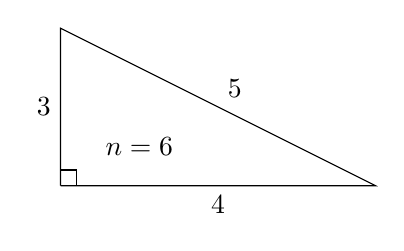
\begin{tikzpicture}[xscale=4, yscale=2]
		\coordinate (O) at (0,0);
		\coordinate (A) at (1,0);
		\coordinate (B) at (0,1);
		\coordinate (M) at (0.25, 0.25);
		\draw (O) -- node[auto,swap]{$4$} 
		(A) -- node[auto,swap]{$5$}
		(B) -- node[auto,swap]{$3$} (O);
		\draw (M) node[auto]{$n=6$};
		\coordinate (X1) at (0,0.1);
		\coordinate (X2) at (0.05,0.1);
		\coordinate (X3) at (0.05,0);
		\draw (X1) -- (X2) -- (X3);
		\end{tikzpicture}
	\end{figure*}\\
	Dit is de driehoek met een oppervlakte van $157$: \cite{Koblitz}[p.5]
	\begin{figure*}[h!]
		\centering
		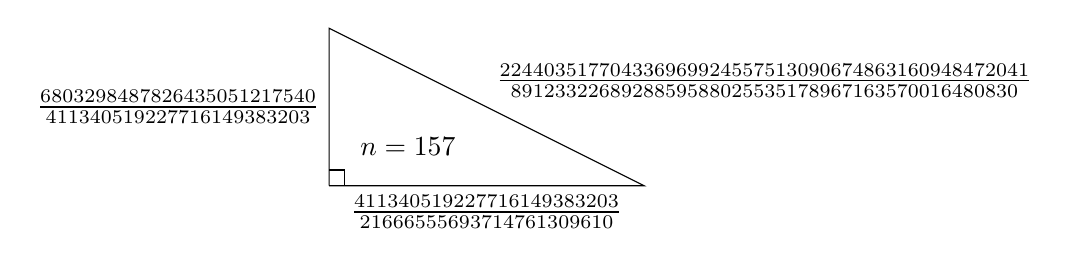
\begin{tikzpicture}[xscale=4, yscale=2]
		\coordinate (O) at (0,0);
		\coordinate (A) at (1,0);
		\coordinate (B) at (0,1);
		\coordinate (M) at (0.25, 0.25);
		\draw (O) -- node[auto,swap]{$\frac{411340519227716149383203}{21666555693714761309610}$} 
		(A) -- node[auto,swap]{$\frac{224403517704336969924557513090674863160948472041}{8912332268928859588025535178967163570016480830}$}
		(B) -- node[auto,swap]{$\frac{6803298487826435051217540}{411340519227716149383203}$} (O);
		\draw (M) node[auto]{$n=157$};
		\coordinate (X1) at (0,0.1);
		\coordinate (X2) at (0.05,0.1);
		\coordinate (X3) at (0.05,0);
		\draw (X1) -- (X2) -- (X3);
		\end{tikzpicture}
	\end{figure*}


	\section{Congruente getallen vinden}
	Voor dit hoofdstuk hebben we gebruik gemaakt van \cite{Koblitz}[p.3-4].\\
	We weten dat een congruent getal $n$ een geheel getal is als oppervlakte van een driehoek met rationale zijden. We willen nu graag weten welke getallen $m\in\NN$ voldoen aan de definitie van een congruent getal. Als we dat willen doen met de kennis van nu, moeten we voor elke $m$ gaan kijken of we een driehoek kunnen vinden met zijden in $\QQ$ zodat de oppervlakte van deze driehoek gelijk is aan $m$. Het is niet moeilijk om te bedenken dat dat een onmogelijke zaak is, zelfs als we de computer laten rekenen. Dus moeten we opzoek gaan naar een manier om het aantal mogelijke getallen $m\in\NN$ te verminderen. Om te kijken hoe we dat kunnen doen, kijken we eerst naar de volgende driehoek:
	\begin{figure}[h!]
		\centering
		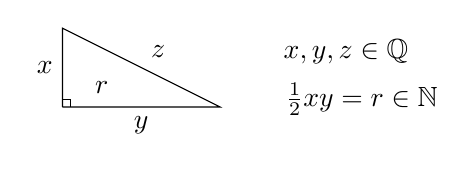
\begin{tikzpicture}[xscale=2, yscale=1]
		\coordinate (O) at (0,0);
		\coordinate (A) at (1,0);
		\coordinate (B) at (0,1);
		\coordinate (M) at (0.25, 0.25);
		\draw (O) -- node[auto,swap]{$y$} 
		(A) -- node[auto,swap]{$z$}
		(B) -- node[auto,swap]{$x$} (O);
		\draw (M) node[auto]{$r$};
		
		\coordinate (S) at (1.8, 0.7);
		\draw (S) node[auto]{$x,y,z\in\QQ$};
		\coordinate (N) at (1.9, 0.1);
		\draw (N) node[auto]{$\frac{1}{2}xy=r\in\NN$};
		\coordinate (X1) at (0,0.1);
		\coordinate (X2) at (0.05,0.1);
		\coordinate (X3) at (0.05,0);
		\draw (X1) -- (X2) -- (X3);
		\end{tikzpicture}
	\end{figure}\\
	Dit is een driehoek met zijn zijden in $\QQ$ en zijn oppervlakte in $\NN$. Dit betekent dus dat $r$ een congruent getal is.
	
	We bekijken nu dezelfde driehoek nadat we alle zijden vermigvuldigd hebben met een getal $s\in\NN$. Deze driehoek ziet er dan alsvolgt uit:
	\begin{figure}[h!]
		\centering
		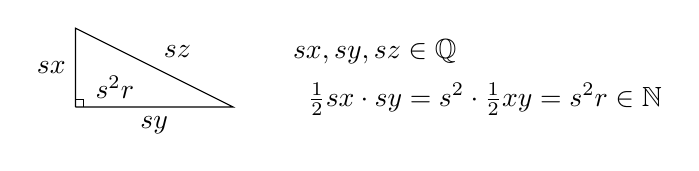
\begin{tikzpicture}[xscale=2, yscale=1]
		\coordinate (O) at (0,0);
		\coordinate (A) at (1,0);
		\coordinate (B) at (0,1);
		\coordinate (M) at (0.25, 0.25);
		\draw (O) -- node[auto,swap]{$sy$} 
		(A) -- node[auto,swap]{$sz$}
		(B) -- node[auto,swap]{$sx$} (O);
		\draw (M) node[auto]{$s^2r$};
		
		\coordinate (S) at (1.9, 0.7);
		\draw (S) node[auto]{$sx,sy,sz\in\QQ$};
		\coordinate (N) at (2.6, 0.1);
		\draw (N) node[auto]{$\frac{1}{2} sx \cdot sy = s^2 \cdot \frac{1}{2}xy = s^2r \in\NN$};
		\coordinate (X1) at (0,0.1);
		\coordinate (X2) at (0.05,0.1);
		\coordinate (X3) at (0.05,0);
		\draw (X1) -- (X2) -- (X3);
		\end{tikzpicture}
	\end{figure}\\
	We zien dat $s^2r\in\NN$ ook een congruent getal is, want de zijden van de driehoek bevinden zich in $\QQ$. Als we nu willen zoeken naar congruente getallen, kunnen we dus ook kijken naar alle kwadraatvrije\footnote{Een kwadraatvrij getal is een getal dat niet deelbaar is door een kwadraat groter dan $1$. Waarbij een kwadraat een getal $k\in\NN$ zodat $\sqrt{k}\in\NN$. \cite{Beukers}} getallen $m'\in\NN$. Namelijk: door het zojuist gegeven voorbeeld zien we dat we $r$ met een willekeurig kwadraat uit $\NN$ kunnen vermenigvuldigen zonder dat het zijn eigenschappen verliest, het is dan nog steeds een congruent getal.

	We hebben nu dus gezien dat we alleen nog maar hoeven te kijken naar kwaadraatvrije getallen. We nemen vanaf nu dus aan dat $n$ een kwaadraatvrij congruent getal is. Dat betekent dat we al een stuk sneller door $\NN$ kunnen gaan om te kijken welke getallen congruent zijn. Sterker nog: er betstaat een algoritme die voor elke $m'\in\NN$ checkt of er een Pythagore\"isch drietal bestaat zodat $m'$ de oppervlakte is van deze driehoek. Als $m'$ congruent is, zet het algoritme deze in een lijst. Helaas weten we niet of een getal dat niet in de lijst staat, ook daadwerkelijk geen congruent getal is. Het kan namelijk ook zo zijn dat het algoritme te lang moest zoeken naar een Pythagore\"isch drietal, waardoor hij het zoeken heeft afgebroken. Dit is dus nog steeds geen optimale manier om naar congruente getallen te zoeken. We zoeken dus eigenlijk nog steeds naar een formule die ons kan vertellen of een getal wel of niet congruent is. Daarvoor introduceren we eerst de stelling van Tunnell:
	\begin{theorem}\label{def:tunnell}
		\cite{Koblitz}[p.212, vertaald] (Tunnell, 1983) Als $n$ een kwadraatvrij en oneven (respectievelijk even) positief geheel getal is en $n$ is de oppervlakte van een rechthoekige driehoek met rationale zijden, dan
		\begin{align}
		\label{vgl:oneven} \#\{x,y,z\in\ZZ \mid n=2x^2+y^2+32z^2\} = \frac{1}{2} \#\{x,y,z\in\ZZ \mid n=2x^2+y^2+8z^2\}\\
		\notag \text{(respectievelijk} \\
		\label{vgl:even} \#\{x,y,z\in\ZZ \mid \frac{n}{2}=4x^2+y^2+32z^2\} = \frac{1}{2} \#\{x,y,z\in\ZZ \mid \frac{n}{2}=4x^2+y^2+8z^2\})
		\end{align}
		Als het zwakke vermoeden van Birch-Swinnerton-Dyer waar is voor de elliptische krommen $E_n:y^2=x^3-n^2x$, dan, omgekeerd, impliceren deze gelijkheden dat $n$ een congruent getal is.
	\end{theorem}
	Deze stelling zegt dat als $n$ een kwadraatvrij en congruent getal is, dan voldoet deze $n$ aan de vergelijkingen (\ref{vgl:oneven}) en (\ref{vgl:even}). Om te checken of een kwadraatvrij getal $m'\in\NN$ congruent is, willen we weten dat de stelling ook de andere kant op werkt. Dit kunnen we alleen aannemen als we het vermoeden van Birch-Swinnerton-Dyer aannemen, een vermoeden over elliptische krommen. Dit is voor nu te ingewikkeld, dus dit zullen we niet verder behandelen. Wat we nu in elk geval hebben is een formule om te kijken of een kwadraatvrij getal $m'\in\NN$ congruent is of niet en dat is waar we naar zochten.
	
	
	\section{Presentaties van congruente getallen}
	We weten al dat ieder congruent getal afhangt van een Pythagore\"isch drietal, welke de presentatie wordt genoemd. Maar is dat een uniek drietal? En zo niet, hoeveel presentaties zijn er dan? Dat zijn de vragen waar we nu naar gaan kijken.\\
	
	Belangrijk is dat we eerst op \'e\'en lijn zitten, aangaande wat precies een Pythagore\"isch drietal is. Hier is een Pythagore\"isch drietal van de vorm $(x,y,z)$, waarbij $x,y,z\in \QQ_{>0}$ en $x^2 + y^2 = z^2$. Het bijbehorende congruente getal noemen we $N$, waarbij uiteraard geldt dat $N\in \QQ_{>0}$ (immers, $N = xy / 2$).\\
	
	Het is dus ook niet moeilijk te zien dat een congruent getal meerdere presentaties kan hebben. Neem bijvoorbeeld het getal 210, een presentatie daarvan is $(20,21,29)$, immers $(20\cdot 21)/2 = 210$. Een andere presentatie is $(12,35,37)$. En hoewel dit slechts \'e\'en getal is, is het desalniettemin zeer aannemelijk dat ieder congruent getal meerdere presentaties heeft. Sterker nog, ieder congruent getal heeft oneindig veel presentaties.\\
	
	Met de huidige definitie van ``presentatie'' is dat moeilijk na te gaan. Om het allemaal wat makkelijker te maken, gebruiken we een nieuwe definitie, gebaseerd op {\color{red}de stelling van Euclides}. We kiezen het positieve gehele getal $D$ dan zo dat $N=m\cdot n \cdot (m-n)^2/D^2$ een primitief congruent getal is. Hierbij zijn $m$ en $n$ zoals in de stelling van Euclides. (Ter herinnering: $m>n$, $ggd(m,n) = 1$ en $m+n$ is oneven.) Daarnaast geldt dat $x = m^2 - n^2$, $y = 2mn$ en $z = m^2 + n^2$.) In dit geval is de presentatie van het congruente getal dan $((m,n),D,N)$. Immers $D^2N = m\cdot n \cdot (m-n)^2$ en $xy/2 = D^2N$.\\
	
	Om nu te bewijzen dat ieder congruent getal oneindig veel presentaties heeft, moeten we eerst wat rekenwerk doen. We defini\"eren eerst:
	\begin{equation}
		U:= z^2=(m^2+n^2)^2, \qquad V:= 2xy=2(m^2-n^2)2mn
	\end{equation}
	Dit zijn de bouwstenen waar we straks een nieuwe presentatie mee gaan vormen voor ons congruente getal. Dat doen we als volgt:
	\begin{align}
			U\cdot V \cdot (U-V) \cdot (U+V)=\\
			z^2\cdot 2xy\cdot (y^2+y^2-2xy)\cdot (x^2+y^2+2xy)=\\
			2xy\cdot z^2\cdot (x-y)^2\cdot (x+y)^2=\\
			\{2\cdot z\cdot D\cdot (x-y)\cdot (x+y)\}^2\cdot N
	\end{align}
	We hebben zo een nieuwe presentatie gevonden van $N$, waarbij een nieuw Pythagore\"isch drietal hoort (voor het gemak $(a,b,c)$ genoemd). Hierbij geldt:
	\begin{equation}
		U'=c^2, \qquad V'=2ab, \qquad E= \mid \{2\cdot z\cdot D\cdot (x-y)\cdot (x+y)\} \mid
	\end{equation}
	Wat opvalt is dat $E>D$.\\
	
	We kunnen deze methode herhalen met $U'$, $V'$ en $E$, en zo weer een nieuwe presentatie vinden. Met die nieuwe presentatie kunnen we weer een nieuwe presentatie vinden, enzovoort. In feite kunnen we het dus oneindig vaak herhalen, waarbij we steeds een nieuwe presentatie vinden. Ergo: ieder congruent getal bevat oneindig veel presentaties.
	
	
	\section{Samenvatting}
	
	
	\bibliographystyle{plain}
	\bibliography{bib}
\end{document}

%	\section{Stellingen}
%	
%	\begin{theorem}
%		\cite{Koblitz}[p.212] (Tunnell, 1983) If $n$ is a squarefree and odd (respectively, even) positive integer ans $n$ is the area of a right triangle with rational sides, then
%		\begin{align}
%		\#\{x,y,z\in\ZZ \mid n=2x^2+y^2+32z^2\} = \frac{1}{2}\#\{x,y,z\in\ZZ \mid n=2x^2+y^2+8z^2\}\\
%		\notag \text{(respectively, } \\
%		\#\{x,y,z\in\ZZ \mid \frac{n}{2}=4x^2+y^2+32z^2\} = \frac{1}{2}\#\{x,y,z\in\ZZ \mid \frac{n}{2}=4x^2+y^2+8z^2\})
%		\end{align}
%		If the weak Birch-Swinnerton-Dyer conjecture is true for the elliptic curves $E_n:y^2=x^3-n^2x$, then, conversely, these equalities imply that $n$ is a congruent number.
%	\end{theorem}
%	
%	\begin{proposition}
%		\cite{Koblitz}[p.4] Let $n$ be a fixed squarefree positive integer. Let $X,Y,Z,x$ always denote rational numbers, with $X<Y<Z$. There is a one-to-one correspondence between right triangles with legs $X$ and $Y$, hypotenuse $Z$, and area $n$; and numbers $x$ for which $x$, $x+n$, and $x-n$ are each the square of a rational number. The correspondence is:
%		\begin{align*}
%		X,Y,Z\rightarrow x &= (Z/2)^2 \\
%		x\rightarrow X &= \sqrt{x+n} - \sqrt{x-n}, Y = \sqrt{x+n}+\sqrt{x-n}, Z = 2\sqrt{x}.
%		\end{align*}
%		In particular, $n$ is a congruent number if and only if there exists $x$ such that $x$, $x+n$, and $x-n$ are squares of rational numbers.
%	\end{proposition}